\فصل{نتایج}
\label{chap:results}

\قسمت{تشکیل آرایش چندذره‌ای با طراحی رهاسازی}
\label{sec:results-particle-formation}

آرایش ذرات در کانال مستطیلی دوبعدی به‌صورت عددی بررسی شد.
هندسه و مدل ذره مطابق بخش~\ref{sec:theory-particle-formation} هستند.
همهٔ مکان‌ها، زمان‌ها و فاصله‌های این بخش بی‌بعد هستند.
در هر حالت، هدف رسیدن هم‌زمان مراکز ذرات به نقاط مشخص بود.
خطای نهایی و کمینهٔ فاصله طبق رابطهٔ~\eqref{eq:validation-formation-errors} محاسبه شدند.

\زیرقسمت{تشکیل یک آرایش ساده}
\label{sec:results-formation-triangle}

مثلث، نمونهٔ پایه برای بررسی آرایش با سه ذره است.
دو ذره از دیوارهٔ پایین و یک ذره از بالا رها شدند.
مکان رهاسازی هر ذره روی دیوارهٔ خودش مستقل انتخاب شد.
دو ذرهٔ پایین تقریباً در زمان $t^*=0.2500$ رها شدند.
ذرهٔ بالا در زمان $t^*=0.2894$ رها شد.
هر سه مسیر در زمان هدف $T^*=0.3462$ ارزیابی شدند.

دو پنل نخست شکل~\ref{fig:results-formation-basic} مسیرها و مراکز نهایی مثلث را نشان می‌دهند.
این نمونه با تنظیمات اجرای پیشین و وزن‌های ثابت دوباره محاسبه شد.
بیشینهٔ خطای نهایی در میدان شبکه برابر $2.67\times10^{-9}$ بود.
در میدان تحلیلی، این خطا به $9.08\times10^{-7}$ رسید.
کمینهٔ فاصلهٔ مراکز در هر دو بازپخش حدود $0.12990$ بود.
این فاصله از آستانهٔ پذیرش $0.026$ بیشتر بود.

\begin{figure}[htbp]
\centering
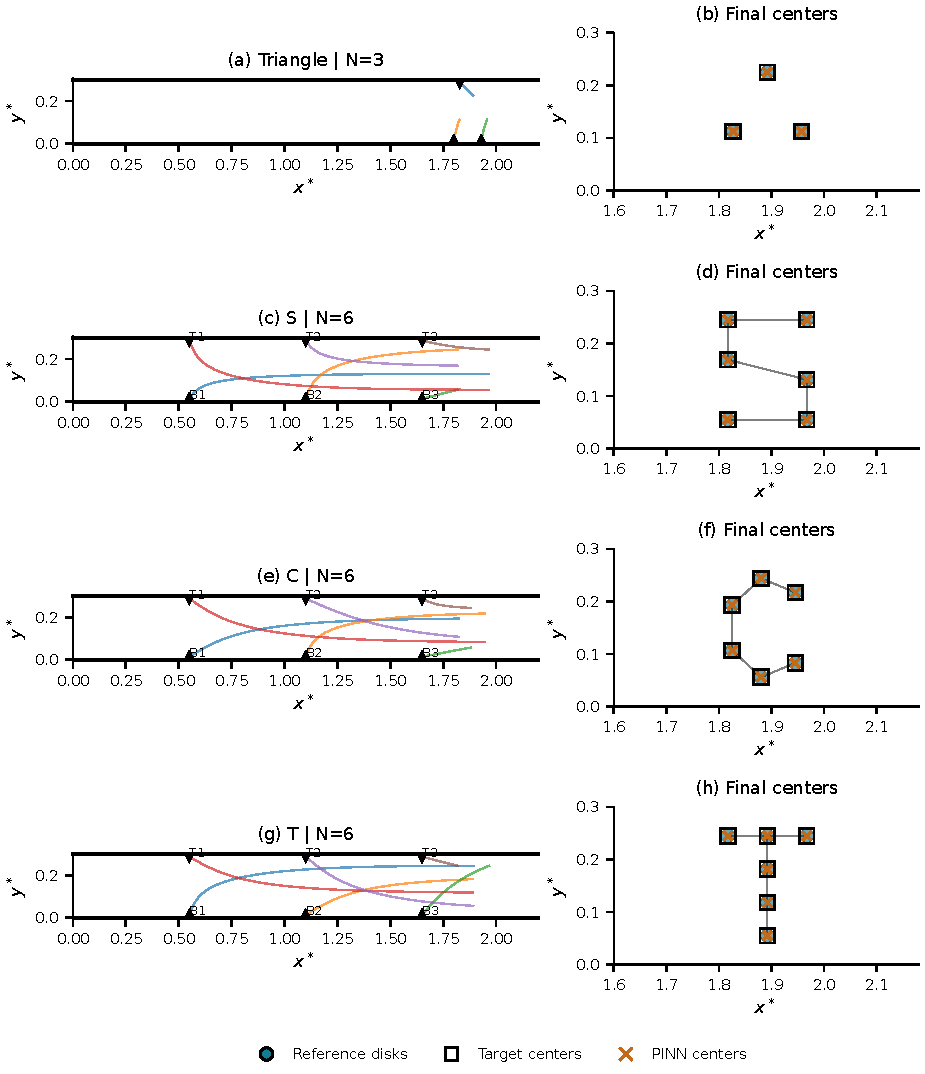
\includegraphics[width=0.95\textwidth,height=0.75\textheight,keepaspectratio]{figs/chapter4/formation-basic-cases.pdf}
\caption{مسیر رهاسازی و مراکز نهایی مثلث و حروف \lr{S}، \lr{C} و \lr{T}.}
\label{fig:results-formation-basic}
\end{figure}

\زیرقسمت{تشکیل حروف \lr{S}، \lr{C} و \lr{T} با شش ایستگاه ثابت}
\label{sec:results-formation-letters}

در هر دیواره، سه ایستگاه در $x^*=0.55,\,1.10,\,1.65$ قرار داشتند.
برای هر حرف، از هر ایستگاه یک ذره رها شد.
سرعت اولیه و زمان رهاسازی برای هر ذره جداگانه تعیین شدند.
سه ردیف پایانی شکل~\ref{fig:results-formation-basic} مسیرهای حروف را نشان می‌دهند.
مراکز نهایی در نمای نزدیک با نقاط هدف مقایسه شده‌اند.

جدول~\ref{tab:results-formation-letters} خطای نهایی و کمینهٔ فاصله را گزارش می‌کند.
بیشینهٔ خطای مرجع در میان حروف، متعلق به حرف \lr{S} بود.
حرف \lr{T} در هر دو بازپخش کمترین فاصلهٔ مراکز را داشت.
کمینهٔ فاصلهٔ مرجع این حرف حدود $0.02746$ بود.
هر سه برنامه در بازپخش عددی معیارهای پذیرش را برآورده کردند.

\begin{table}[htbp]
\centering
\small
\setlength{\tabcolsep}{5pt}
\caption{خطای نهایی و کمینهٔ فاصلهٔ بی‌بعد برای سه حرف.}
\label{tab:results-formation-letters}
\begin{tabular}{@{}lccccc@{}}
\hline
حرف & $T^*$ & $E_{\max,\mathrm{PINN}}^*$ & $E_{\max,\mathrm{ref}}^*$
& $d_{\min,\mathrm{PINN}}^*$ & $d_{\min,\mathrm{ref}}^*$ \\
\hline
\lr{S} & $2.3875$ & $2.073\times10^{-8}$ & $3.768\times10^{-4}$ & $0.0335802$ & $0.0336059$ \\
\lr{C} & $1.8674$ & $1.121\times10^{-8}$ & $1.948\times10^{-4}$ & $0.0348533$ & $0.0348257$ \\
\lr{T} & $2.2739$ & $1.141\times10^{-8}$ & $2.877\times10^{-4}$ & $0.0274005$ & $0.0274613$ \\
\hline
\end{tabular}
\end{table}

اندیس \lr{PINN} به بازپخش با میدان شبکه اشاره دارد.
اندیس \lr{ref} بازپخش مستقل با میدان تحلیلی پوازوی را مشخص می‌کند.
مقدار $T^*$ زمان هدف همان آرایش است.

\زیرقسمت{آرایش اردک و بازپخش مستقل برنامه‌های رهاسازی}
\label{sec:results-formation-ducks}

چهار برنامهٔ ذخیره‌شده برای آرایش اردک دوباره بازپخش شدند.
حالت‌های ۲۰ و ۴۲ ذره‌ای از شش ایستگاه ثابت استفاده کردند.
در این حالت‌ها، هر ایستگاه می‌توانست چند ذره رها کند.
در حالت‌های ۲۸ و ۶۴ ذره‌ای، مکان رهاسازی هر ذره آزاد بود.
هر برنامه با میدان شبکه و میدان تحلیلی پوازوی بازپخش شد.
برنامهٔ رهاسازی هر حالت در هر دو بازپخش یکسان بود.

شکل~\ref{fig:results-formation-ducks} آرایش‌ها را در زمان هدف هر برنامه نشان می‌دهد.
دیسک‌ها اندازهٔ ذرات را با مقیاس هندسی کانال نشان می‌دهند.
جدول~\ref{tab:results-formation-ducks} خطای نهایی و کمینهٔ فاصله را مقایسه می‌کند.

\begin{figure}[htbp]
\centering
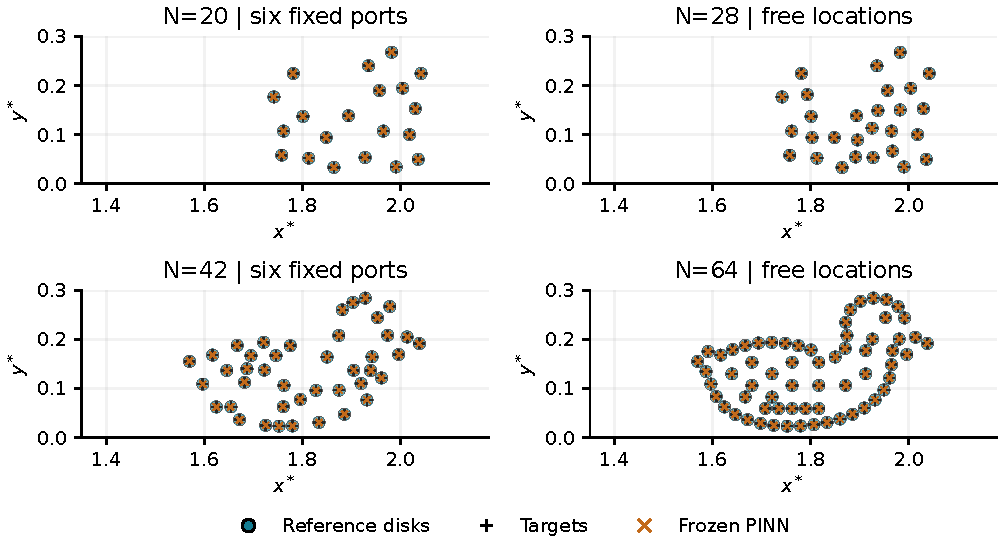
\includegraphics[width=0.95\textwidth]{figs/chapter4/formation-duck-replays.pdf}
\caption{چهار آرایش اردک در زمان هدف برنامه‌های رهاسازی.}
\label{fig:results-formation-ducks}
\end{figure}

\begin{table}[htbp]
\centering
\small
\setlength{\tabcolsep}{5pt}
\caption{مقایسهٔ بی‌بعد بازپخش شبکه و میدان تحلیلی برای آرایش اردک.}
\label{tab:results-formation-ducks}
\begin{tabular}{@{}clcccc@{}}
\hline
$N$ & نوع رهاسازی & $E_{\max,\mathrm{PINN}}^*$ & $E_{\max,\mathrm{ref}}^*$
& $d_{\min,\mathrm{PINN}}^*$ & $d_{\min,\mathrm{ref}}^*$ \\
\hline
$20$ & شش ایستگاه ثابت & $7.243\times10^{-4}$ & $7.616\times10^{-4}$ & $0.0296120$ & $0.0293893$ \\
$28$ & مکان آزاد & $2.939\times10^{-6}$ & $1.452\times10^{-6}$ & $0.0286904$ & $0.0286904$ \\
$42$ & شش ایستگاه ثابت & $6.503\times10^{-4}$ & $6.621\times10^{-4}$ & $0.0262260$ & $0.0260481$ \\
$64$ & مکان آزاد & $3.456\times10^{-4}$ & $3.456\times10^{-4}$ & $0.0262883$ & $0.0262883$ \\
\hline
\end{tabular}
\end{table}

هر چهار برنامه در بازپخش عددی پذیرفته شدند.
آرایش ۴۲ذره‌ای کمترین حاشیهٔ فاصله را در میان چهار برنامه داشت.
در بازپخش مرجع، حاشیهٔ این آرایش حدود $4.81\times10^{-5}$ بود.
این حاشیه از اختلاف کمینهٔ فاصله میان دو بازپخش کوچک‌تر بود.
این اختلاف اهمیت بازپخش مستقل را برای برنامه‌های نزدیک آستانه نشان می‌دهد.

% Keep the final comparison paragraph on the preceding text page.
\enlargethispage{2\baselineskip}
در این چهار نمونه، تعداد ذرات و نوع رهاسازی هم‌زمان تغییر می‌کنند.
بنابراین مقایسهٔ آن‌ها عملکرد چهار برنامهٔ مشخص را توصیف می‌کند.
آرایش‌های گزارش‌شده به زمان هدف هر برنامه تعلق دارند.
